\section{\acrlong{fer}}
\subsection{Data Collection}
To recognize emotions in images, the kaggle dataset \textbf{FER2013} \cite{FER2013} will be used. This dataset was prepared by Pierre-Luc Carrier and Aaron Courville as part of an ongoing research project and contains $35,887$ images, displaying the emotions anger, fear, sadness, neutralilty, happiness, surprise and disgust. Hereby, Figure \ref{fig:emo-distribution} represents the corresponding distribution of those emotions. Moreover, this dataset includes people from different genders, ethnicities and ages. Furthermore, the FER2013 dataset is handled according to the terms of the Open Database License (ODbL), which states the following: ``The Licensor grants to You a worldwide, royalty-free, non-exclusive, perpetual, irrevocable copyright license to do any act that is restricted by copyright over anything within the Contents, whether in the original medium or any other. These rights explicitly include commercial use, and do not exclude any field of endeavour [...].'' \cite{odbl} We may also use additional datasets provided by kaggle or other sources.

\begin{figure}[h!]
\centering
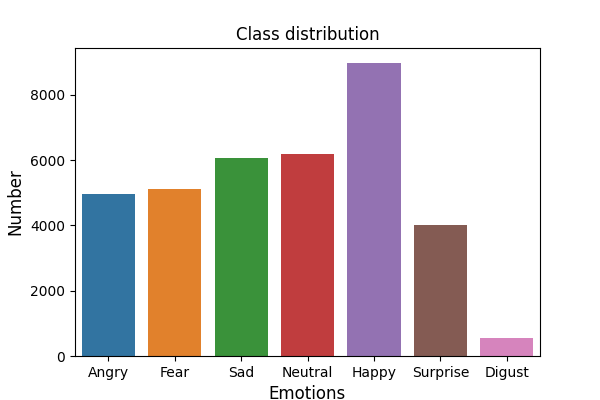
\includegraphics[scale=0.8]{barplot1.png}
\caption{Barplot of the distribution of the different classes of emotion.}\label{fig:emo-distribution}
\end{figure}

\subsection{Data Preprocessing}
Before using the datasets, they will be preprocessed to exclude irrelevant images/emotions. Data preprocessing includes reducing different types of noises, resizing the picture, and aligning facial features. The method typically used to achieve the results is the eye selection method. Figure \ref{fig:emo-distribution} provides an example image of the different facial expressions with their corresponding labeled emotion. 
The \textit{FER2013} dataset provides preprocessed and labeled grayscaled images of facial emotions. We will however implement a pipeline to process new images. This will contain the following steps. The first step is to convert the (RGB) color image to a grayscale image. The colors in images can often contain clutter and hinder the model form detecting faces accurately. After the grayscale conversion, the next step is to crop and align the images, so that we are left only with the face. We should mention, that in this step we have to consider the resolution of the image and if the crop is still usable after the crop. The next step is to de-noise the image and apply filtering. De-noising the image will amplify and enhance the meaningful features of an image while reducing background noise.   Filtering is the process of altering properties of the image, for example contrast and saturation. For grayscaling and cropping the image we will use the OpenCV library.

\begin{figure}[h]
\centering
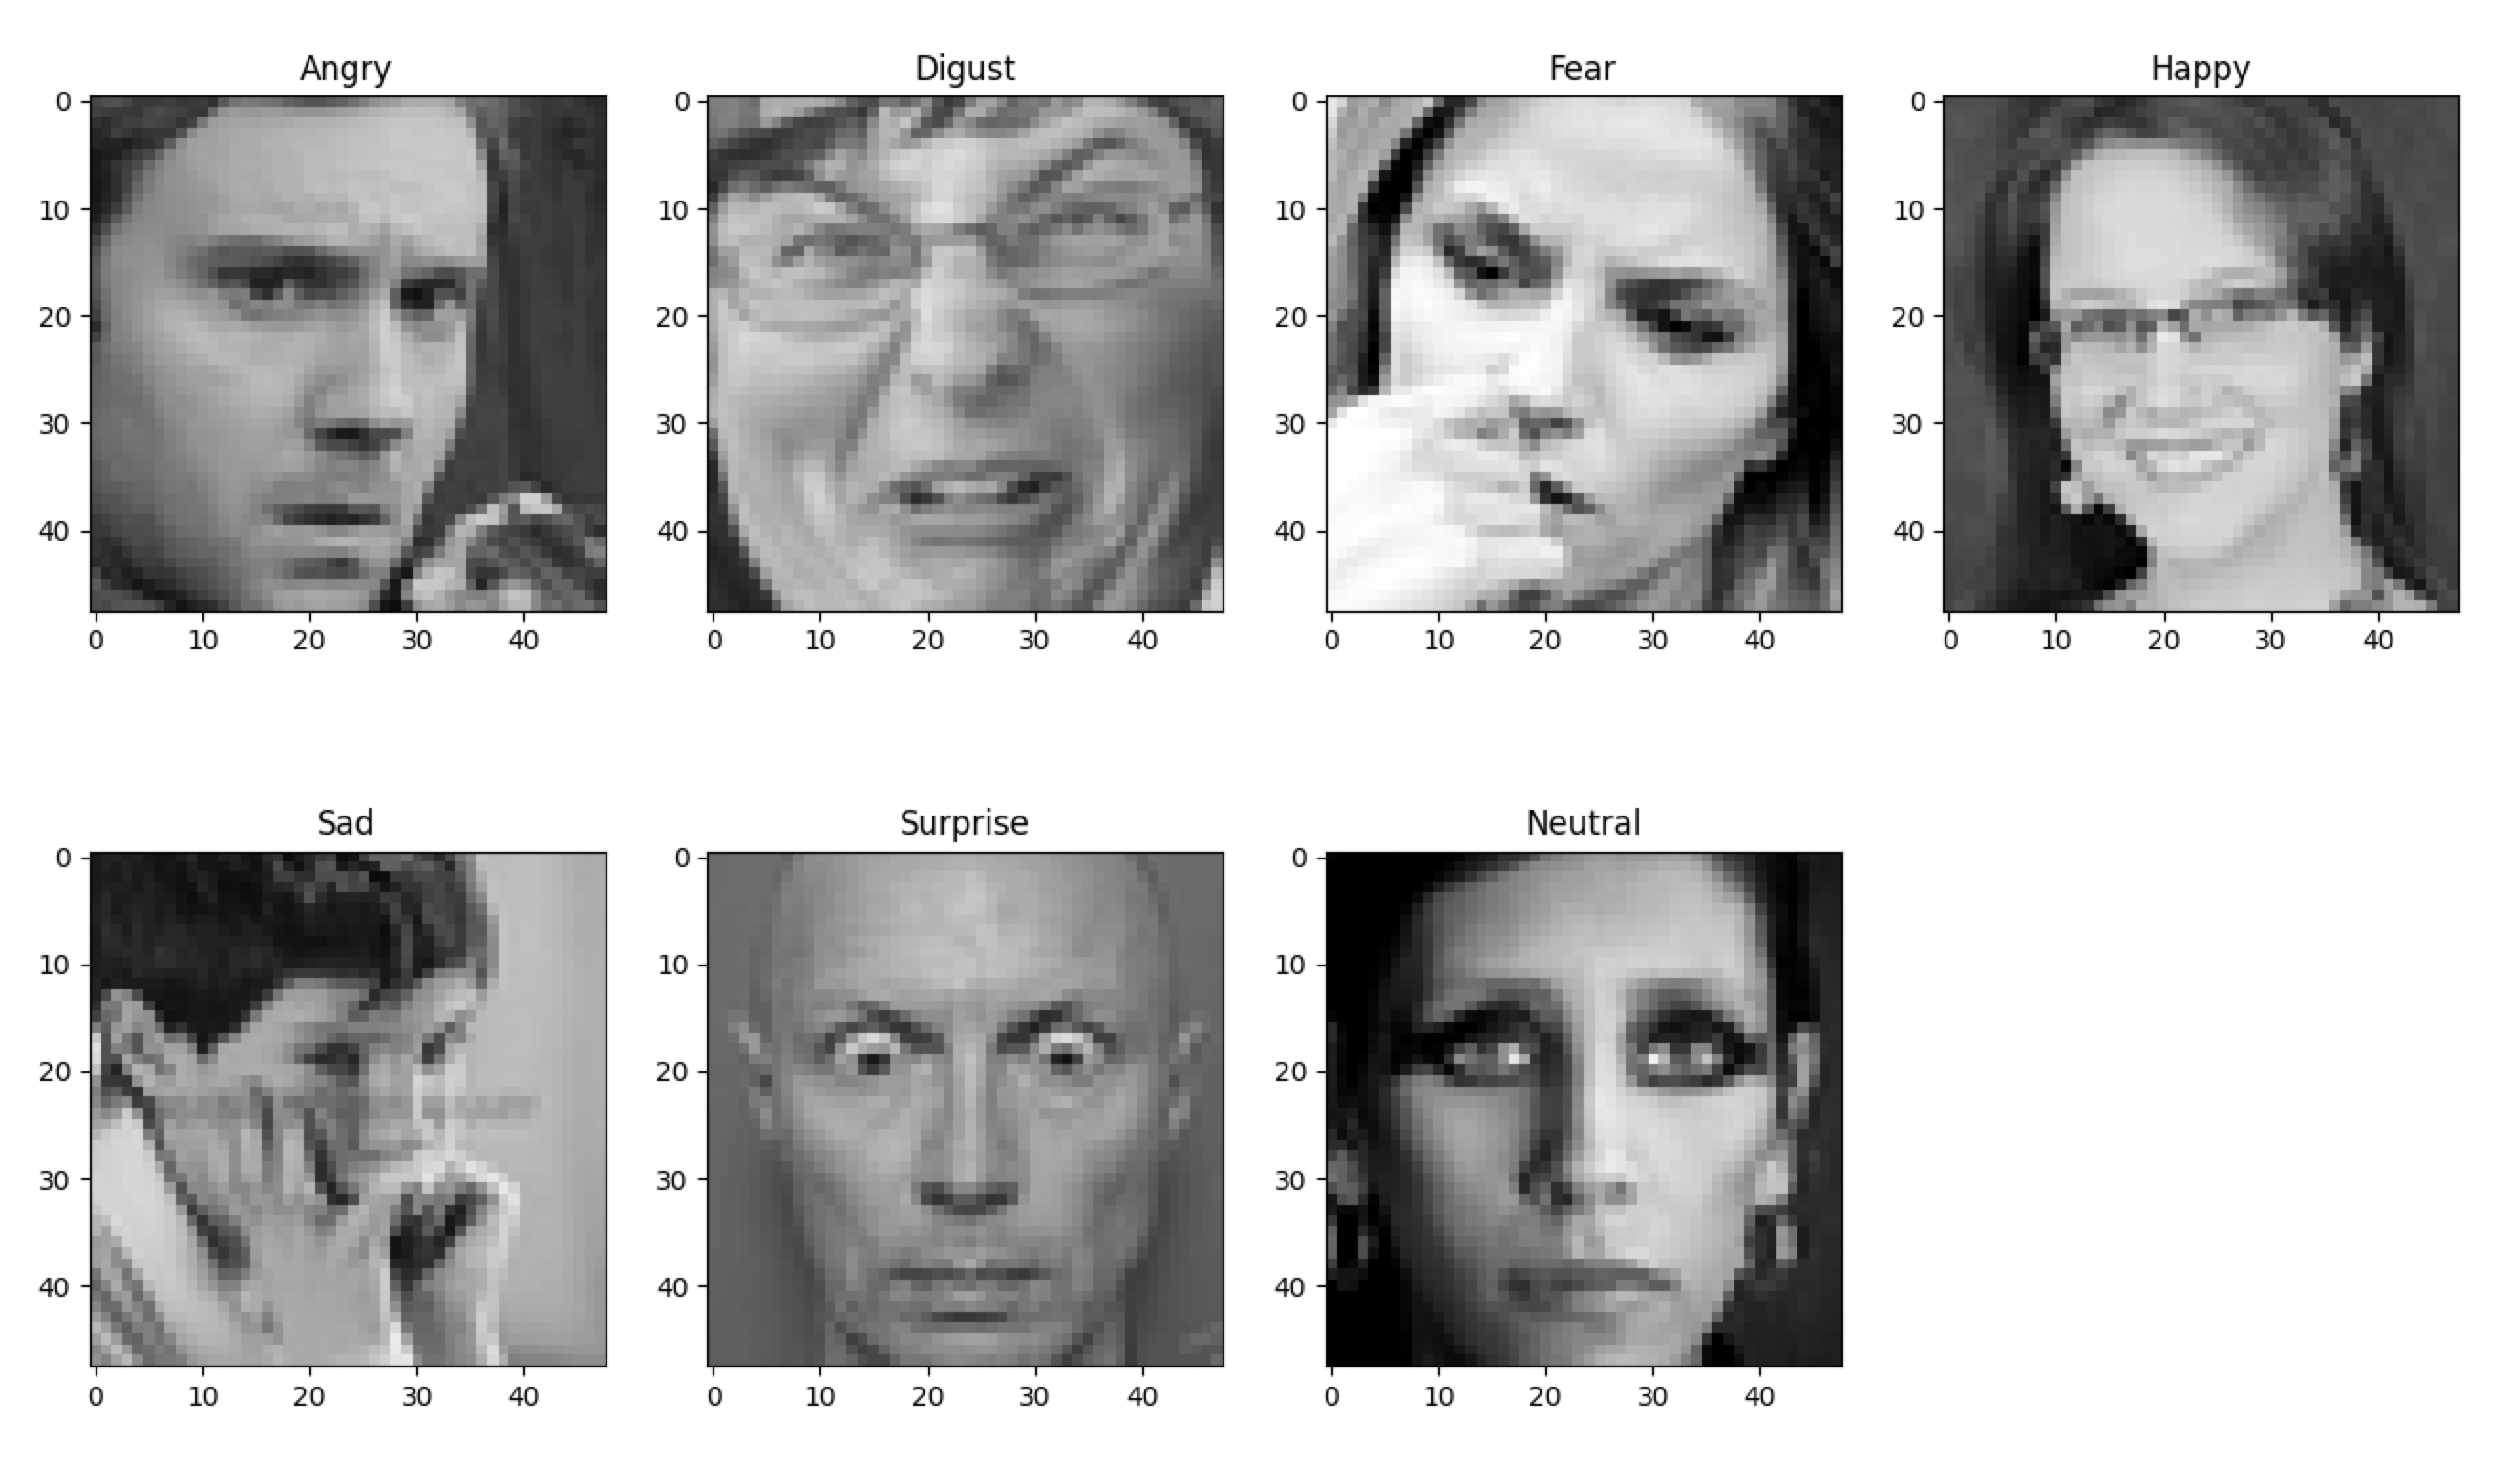
\includegraphics[width=0.9\textwidth]{faces1.png}\\
\caption{Facial expressions with corresponding emotions. \cite{FER2013}}\label{fig:faces}
\end{figure}
